\subsubsection{Open Access Publishing}
\label{ict:stamer}
\index{Stamerjohanns, Heinrich}

\paragraph{Research Team}
Heinrich Stamerjohanns (Head of CS Labs), also member of KWARC
Research Team, see~\ref{ict:modeling:kohlhase}.\\

With the fundamental change of the existing paper publication system
towards networked digital publications a variety of new possibilities arise
to overcome the existing technical constraints of scientific documents
in order to increase the effectiveness of scientific research.

Scientific exchange may be improved in various ways:
\begin{myitemize}
\item by giving free and and unrestricted access (Open Access) to
the results of scientific research
\item by enabling access not only to text and pixeled images
but to complete sources (data, programs) of the obtained results
\item by semantically annotating content in order to improve
the searchability by machines.
\end{myitemize}

\paragraph{Highlights}

We proposed a content markup language for physics realized by
extending the OMDoc format by an infrastructure for the principal
concepts of physics: observables, physical systems, and experiments.
The formalization of the description of physics observables follows
the structural essence of the operational theory of physics
measurements. The representational infrastructure for systems and
experiments allow to capture the distinctive practice of physics:
natural laws are supported by evidence from experiments which are
described, disseminated and reproduced by others.

In a collaboration with Prof. Jeltsch we are also developing tools
to dynamically publish generated data that will help to understand the genetic
and epigenetic basis for DNA-methylation variation in the human genome,
to asses sequence specificity of DNA-methylation patterns in normal tissues.

\begin{figure}[ht]
  \begin{center}
    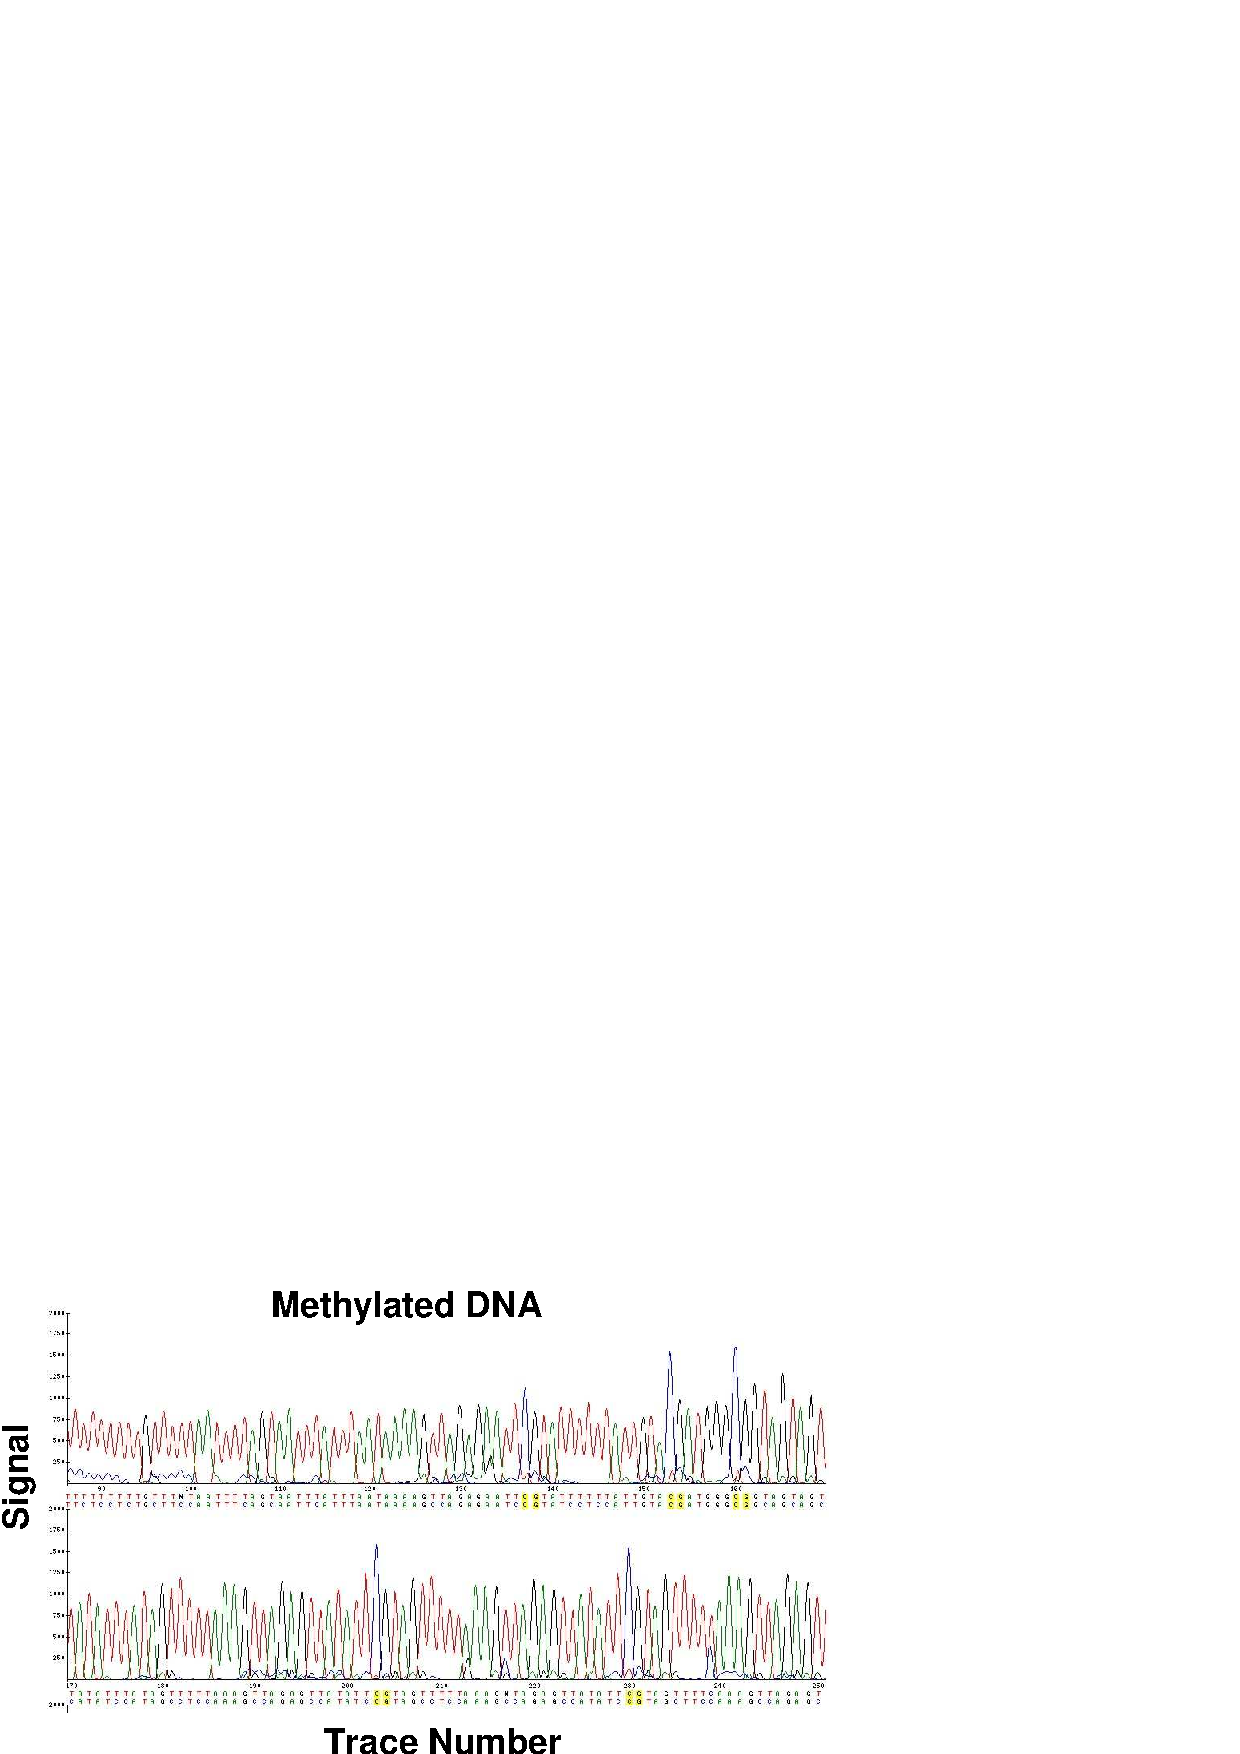
\includegraphics[width=\hsize,bb=0 0 390 230]{stamerjohanns-fig1.pdf}
    \caption{Dynamically created content of the analysis of methylated DNA. Other
    researches do not only have access to images, but to full research data.}\label{fig:stammerjohanns}
   \end{center}
\end{figure}

As a member of the Deutsche Initiative f\"ur Netzwerkinformation (DINI)
Working Groups \textsl{E-Publications}
and \textsl{Open Archives}, we are trying to establish common standards
for Scientific Institutional Repositories.

\paragraph{Collaborations}
\begin{enumerate}
    \item {\sl International University  Bremen} \\
            Prof. M. Kohlhase \\
            Extending OMDOC to PhysML, ArXiv conversion     \\
            Prof. A. Jeltsch \\
            Dynamic publishing of SMP Epigenetics Data

    \item {\sl ISN Oldenburg} \\
            Prof. E.R. Hilf \\
            Extending OMDOC to PhysML\\
            Citation Linking and Indexing

    \item {\sl DINI Working Groups} \\
            Certificate for Institutional Repositories

\end{enumerate}

%\paragraph{Publications}
\nocite{HilKohSta:copmem06,DINI06}
